% Evaluation

\chapter{Results and Evaluation} % Main chapter title

\label{Chapter6} % For referencing the chapter elsewhere, use \ref{Chapter4} 

\lhead{Chapter 6. \emph{Results \& Evaluation}} % This is for the header on each page - perhaps a shortened title

%----------------------------------------------------------------------------------------


\section{Quantitative}
\vspace{10pt}

\subsection{Evaluation of Mood Detection system}

\begin{figure}[t]
    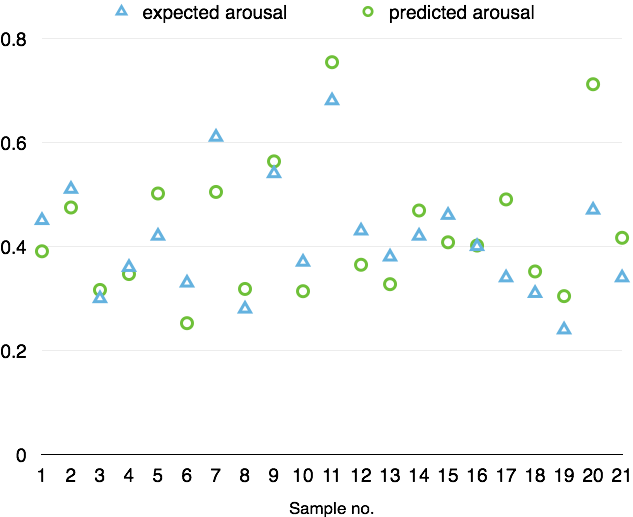
\includegraphics[width=0.7\textwidth]{Figures/finalarousal}
    \centering

  \caption{A plot of the expected and predicted .}
  \label{fig:anneval}
\end{figure}


We wanted to use neural networks to calculate valence and arousal ratings of songs using audio features we extract. 

We computed the mean error between participant ratings and network-predicted outputs across all segments of all test melodies. The network's performance total RMSE was 0.088954243616 on scale from 0 to 1 or 21.62\%.
The network predicted at an average accuracy of 78.38\% for all 20 segments. The plot of the expected and predicted values can be seen in Figure \ref{fig:anneval}.
These results are more promising than ones of Yang and Lin \cite{mood}, where their $R^2$ scored 58.3\% for arousal and 28.1\% for valence.


\begin{figure}[t]
    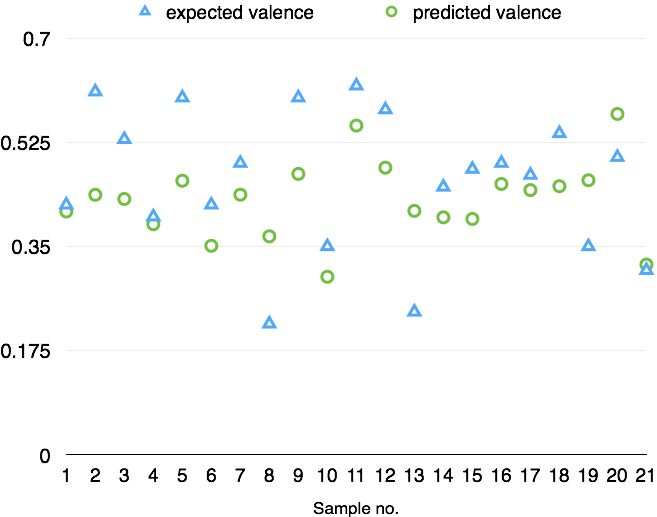
\includegraphics[width=0.7\textwidth]{Figures/finalvalence}
    \centering

  \caption{A plot of the expected and predicted valence.}
  \label{fig:anneval}
\end{figure}


Results from the static network indicate that a network can be trained to identify statistical consistencies across audio features abstracted from music and satisfactorily predict valence/arousal values that closely match mean participant ratings.


\begin{table}
\begin{center}
\begin{tabular}{| c | c | c | c | } \hline 
 expected arousal & expected valence & predicted arousal & predicted valence \\ \hline \hline

0.45  & 	0.42  &  0.390444 &  0.408524   \\ \hline
0.51	&  0.61  &  0.474538 & 0.436625   \\ \hline
0.3    &  0.53  &  0.316230 & 0.429643   \\ \hline
0.36	&  0.4    &  0.346713 & 0.387249   \\ \hline
0.42	&  0.6    &  0.501414 & 0.460295   \\ \hline
0.33	&  0.42  &  0.252398 & 0.350910  \\ \hline
0.61	&  0.49  &  0.504392 & 0.436785   \\ \hline
0.28	&  0.22  &  0.318096 & 0.366836   \\ \hline
0.54	&  0.6    &  0.563120 & 0.471717   \\ \hline
0.37	&  0.35  &  0.313782 & 0.298909   \\ \hline
0.68  &  0.62  &  0.753534 & 0.552922   \\ \hline
0.43	&  0.58  &  0.364568 & 0.482194   \\ \hline
0.38	&  0.24  &  0.327288 & 0.409628   \\ \hline
0.42  &  0.45  &  0.468762 & 0.398749   \\ \hline
0.46  &  0.48  &  0.407701 & 0.396029   \\ \hline
0.4    &  0.49  &  0.401469 & 0.454892   \\ \hline
0.34  &  0.47  &  0.490065 & 0.444592   \\ \hline
0.31  &  0.54  &  0.351714 & 0.451086   \\ \hline
0.24  &  0.35  &  0.304314 & 0.461078   \\ \hline
0.47	&  0.5    &  0.711224 & 0.572459   \\ \hline
0.34	&  0.31  &  0.416320 & 0.319491   \\ \hline


\end{tabular}
\caption{Table showing the root mean square error for training the network for given number of nodes in the hidden layer.}
\label{table:rsmetablefinal}
\end{center}
\end{table}


\subsection{Melody Extraction Testing}
To evaluate our implementation of the melody extraction algorithms we can use the technique used at Music Information Evaluation eXchange, described in section 2.4.3 of the report. In particular, we can compare the performance of our implementation when tested on the samples used during MIREX to the official statistics presented in papers \cite{salamon, comparison}.

Another way of evaluating the game is creating a set of songs and generating levels for them. After that a trained Guitar Hero player can play those levels. If the buttons were consistently on time with the notes then the melody extraction and game synchronisation techniques are considered to work.

\section{Qualitative}
Qualitative research is conducted to gain understanding of effects and benefit of the project. They focus on people's own experiences and provide insights and trends in thoughts on a given matter. They can be unstructured or semi-structured, conducted as group discussions, surveys or individual interviews.



\subsection{Questionnaires}
Questionnaires are one of the most common and popular tools to gather data from a large number of people. They generally consist of a limited number of questions that ask participants to rate the effectiveness of various aspects of the activity. The questions should focus on the key points we are trying to evaluate. 

Questionnaires tend to be short in order to reduce the amount of time respondents need to complete them, and therefore increase the response rate. 

We composed questionnaires that are quantitative and generally consist of close-ended questions (tick the box, or scales), as the open ended questions tent to make data analysis and reporting more difficult.

\subsubsection*{Preliminary Research}

Before the design and implementation phase of the project, we conducted a study to determine what features could be desirable in the game. We led a survey among 18 people aged 17-25 asking about their past experience with music rhythm games. 
The questions and the results are presented in the Table \ref{table:preliminaryquestions}. Each of the questions was answered on a scale from 1 to 5, where 1 is a No,  3 is Neutral and 5 is a Yes.

\begin{table}
\begin{center}
\begin{tabular}{| p{8cm} | c | c | c | c | } 																								      \hline 
\textbf{Question} & \textbf{Average} & \textbf{Stdev} & \textbf{Min} & \textbf{Max} 						   \\ \hline \hline
Do you like playing games? & 4.11 & 0.9 & 2 & 5		 					 					 									\\ \hline 
Do you like listening to music? & 4.67 & 0.59 & 3 & 5		 					 					 								\\ \hline 
Do you often play games? & 3.722 & 0.89 & 2 & 5 		 					 					 								\\ \hline 
Have you ever played Guitar Hero or other rhythm music game? & 3.88 & 1.84  & 1 & 5							\\ \hline 
Did you feel like the choice of songs was limiting you? & 3.22 & 1 & 1 & 5 					 							\\ \hline 
Were you able to load in your song of choice in there? & 2. & 1.41 & 1 & 5 					 							\\ \hline 
Would you like to be able to load a song into it? & 4.27 & 0.82 & 3 & 5 				 									\\ \hline 
Did you feel like the game graphics were reflecting the emotions in the song? & 2.78 & 1.06 & 1 & 4 			\\ \hline 
Would you like the game to reflect the emotions in the song? & 3.67 & 0.84 & 3 & 5 	 								\\ \hline 
Was the game reflecting the section of the song you were in? & 2.44 & 1.25 & 1 & 4  								\\ \hline 
Do you feel it would be useful to know what section of the song is currently played? & 3.5 & 0.86 & 2 & 5  	\\ \hline 
\end{tabular}
\caption{Table presenting the results of the preliminary questionnaire.}
\label{table:preliminaryquestions}
\end{center}
\end{table}

As we can see from the Table \ref{table:preliminaryquestions}, the majority of young people surveyed did enjoy playing games to a similar extent. However, the results of the survey tell us that listening to music is almost unanimously beloved activity, with the highest average result and the smallest standard deviation. 
Majority of people play games quite often, but the lower average and standard deviation compared to the first question suggests that there are some people who enjoy playing games a lot but they do not spend that much time doing so, be it due to lack of time or other arrangements. 

When it comes to rhythm-games specific questions, most people have played a game of such type before. A majority of people believed that having a set playlist was limiting their experience, however, there were some who did not mind this that much. However, when asked if the ability to upload their own music would improve their experience, everybody was either neutral of agreed - nobody was against the idea. 

Majority, but no all surveyed believed that the rhythm game they played did not reflect the mood of the song they played, which can be deducted from the average below the neutral value 3 with the maximum value being four, so above the neutral. They believed it would be nice for the game to reflect the emotions in the song, but the need expressed was not as urgent as in case of the upload of their own songs. On the other hand, nobody opposed to such feature, which is reflected by the minimum value given being three.

Finally, we asked the surveyed whether they felt like the game was reflecting the built of the song, notifying them of where in the song they were. Most agreed that the games like that did not contain any sort of visualisation for the song segmentation. Majority of surveyed agreed that such feature would be useful, although a small amount of people believed it would not contribute in any way, answering with 2.

We also had to additional questions asking for suggestions, in case there are other features that could be useful to the game or could make the game more attractive that we missed in our initial market research. 

\subsubsection{Final Research}

For our final research, we demonstrated our game to a group of 8 people aged 18-23 and asked them to fill in a questionnaire to describe their experience and thoughts on the game. Each of the questions was answered on a scale from 1 to 5, where 1 is a No,  3 is Neutral and 5 is a Yes. The questions and the results are presented in the Tables \ref{table:finalquestionsinterface}, .

\begin{table}
\begin{center}
\begin{tabular}{| p{8cm} | c | c | c | c | } 																	  \hline 
 \textbf{Question} & \textbf{Average} & \textbf{Stdev} & \textbf{Min} & \textbf{Max } \\ \hline \hline
 I knew what to do in the game straight away. 				& 4.88 & 0.35 & 4 & 5		   \\ \hline 
 I needed hints to play the game. 								& 2.25 & 1.58 & 1 & 5 	   \\ \hline 
 I needed somebody to tell me how to play the game. 	& 1.13 & 0.35 & 1 & 2  	   \\ \hline 
 I liked the design of the menu. 									& 3.86 & 0.99 & 2 & 5   	   \\ \hline 
 I felt like the game interface was too crowded. 				& 1.38 & 0.51 & 1 & 2 	   \\ \hline 
 I felt like the interface of the menu was too empty.		& 1.75 & 0.89 & 1 & 3		   \\ \hline
 I felt like i knew what each part was supposed to do. 	& 4.75 & 0.46 & 4 & 5		   \\ \hline
\end{tabular}
\caption{Table presenting the results of the final questionnaire concerning the game interface.}
\label{table:finalquestionsinterface}
\end{center}
\end{table}

As we can see, a vast majority found the user interface fairly straightforward. The rest of the interviewed needed hints provided in the game to fully understand the game play and the flow of the use. Almost nobody felt like they needed someone to explain what they are supposed to do in the game. 

More than half of the people liked the design of the menu - almost nobody felt like it was too crowded or too empty. In addition to this, the vast majority of the surveyed believed they could guess the purpose of the elements visible in the interface, with minimum response being 4.

\begin{table}
\begin{center}
\begin{tabular}{| p{8cm} | c | c | c | c | } 																			   \hline 
 \textbf{Question} & \textbf{Average} & \textbf{Stdev} & \textbf{Min} & \textbf{Max }	\\ \hline \hline
 The game was too difficult. 														& 2.86 & 0.83 & 2 & 4 \\ \hline		
 The game was too easy. 															& 1.13 & 0.35 & 1 & 2  \\ \hline
 The buttons felt synchronised with the game. 								& 3.75 & 0.46 & 3 & 4	 \\ \hline
 I noticed the changes in the mood influenced the game interface.	& 3.25 & 1.04 & 1 & 4	 \\ \hline
 I found the structure recognition useful.										& 4.00 & 0.35 & 3 & 5  \\ \hline
 I knew how to quit / pause / resume the game straight away.			& 4.88 & 0.83 & 4 & 5	 \\ \hline
 I knew how I was scored straight away.										& 4.13 & 0.93 & 3 & 5	 \\ \hline
 \end{tabular}
\caption{Table presenting the results of the final questionnaire concerning the gameplay.}
\label{table:finalquestionsgameplay}
\end{center}
\end{table}

The second set of questions was designed to find out about users' thoughts on the game itself. In the survey, we asked what the interviewees thought about the game's difficulty. The results can be seen in Table \ref{table:finalquestionsgameplay}. Nobody believed the game was too easy, with an average answer of 1.13 and maximum one being 2. The majority of the surveyed also thought that the game was not too difficult, although the average response was much closer to neutral. We believe that this is a desirable outcome, as the game is supposed to pose a challenge to the player or they will quickly become bored with it. 

We also focused on the assessment of individual elements that create the game experience and make it stand out from all the publications available on the market. The incorporation of the predominant melody detection as well as the button generation algorithm were referred to in a question about synchronisation between the music and the notes that come up on the screen. Every person asked either agreed or was neutral in response to the question. We believe the variation in the answers is due to different choice of songs the surveyed decided to upload. If the song did not have a one definite predominant melody from a single source, the buttons would become less predictable. 
We are satisfied with this score as the fact that nobody gave it less than 3 implies that the algorithms fulfill their purpose and generate relevant outputs in general.

The next question regarded the mood detection. Although the average response suggests that the users did notice the changes in the visuals triggered by the mood changes in the music, in fact, many people felt indifferent about this feature. When asked what they thought the reason was, they stated they were too focused on trying to ace the buttons to pay attention to the animation in the background.

We also asked about users' opinion on the structure retrieval system and its incorporation. Most people found it useful, claiming it helped them track where in the song they were. We believe the feature was a success as the lowest score it received was a neutral one. 

When asked about the controls, the all the users agreed that they were easy to find and use. In addition to this, they all felt that they new how the scoring worked and what to do to improve their results. 

\begin{table}
\begin{center}
\begin{tabular}{| p{8cm} | c | c | c | c | } 																			   \hline 
 \textbf{Question} & \textbf{Average} & \textbf{Stdev} & \textbf{Min} & \textbf{Max }	\\ \hline \hline
 I think the application does not require previous computer experience to be used properly. & 4.63 & 0.52 & 4 & 5 \\ \hline
 The buttons were designed in such way that the user can quickly become familiar with the game environment. & 4.38 & 0.52 & 4 & 5 \\ \hline
 The screens are well structured and their design is clear, aesthetic and attractive.  & 4.00 & 0.76 & 3 & 5 \\ \hline
 The amount of on-screen texts is not excessive. 	& 5.00 & 0.00 & 5 & 5 \\ \hline
 The fonts are clear and readable. 						& 3.38 & 0.74 & 3 & 5 \\ \hline
 The combination of colours is pleasing. 				& 4.38 & 0.74 & 3 & 5 \\ \hline
 \end{tabular}
\caption{Table presenting the results of the final questionnaire concerning the overall experience when playing the game.}
\label{table:finalquestionsoverall}
\end{center}
\end{table}

The final set of questions given to the surveyed asked them about their overall experience and thoughts on the application. Every person questioned believed to some extent that the application we created does not require the users to have previous computer experience to play - there was no answer below 4. This is really important, especially for a game, which we believe should be available and easy to use to everyone who wants to play it. 

The surveyed also appreciated the design of the buttons claiming their design helped to understand the flow of use.
They also believed that the structure of the screens was logical and visually pleasing. In addition to this, everybody unanimously agreed that the amount of the on-screen text was not excessive. This is encouraging, as very often games repel people by forcing them to read long lines of text. The colour scheme also received a favourable review, scoring an average of 4.38.

Most people believed that the fonts were clear and readable, but a few believed that a small increase in the font size would improve the user experience. 


